%\section{Estruta da tese e   Etapas da Resolução do Problema}
%
%1. Analisar conjunto de dados. Ver nr de contratos, ver nr de procedimentos e nr de tipo de contratos, etc
%
%2. Categorizar as flags de acordo com a facilidade de implementação e valor
%
%3. Focar, numa fase inicial, num conjunto de contratos. Selecionaram-se apenas ajustes diretos e contratos públicos referentes a CPV's que dizem respeito a %serviços de consultoria de IT - 72

%4. Contruiu-se a primeira flag que compara preço base com preço contratual 
%
%5. Construi-se função que verifica se os precos contratuais dentro dos ajustes diretos caem dentro de um intervalo em torno do preco base
%
%6. Nesta mesma função, inclui-se a presença de um parametro de racio para comparar com precobase/precocontratual. Nos casos em que este quociente é mt alto vai ser verificado se ha ou nao presenca de vários lotes no contrato
%
%7. Construcao de uma funcao que vai analisar ajustes diretos. Priemiro verifica quais os ids dos contratos q ultrapassam o valor maximo permitido por lei q é 20k€. Se ultrapssar dispara a flag. Se num ajuste direto nao houver fundamentação é disparada a flag tambem
%
%8. Os ajustes diretos foram ordenados por ordem crescente de nt de celebracao. Comparou-se o nr de ajustes diretos celebrados com o nt de ajustes suspeitos, calculou-se o racio entre os 2. 
%
%9. No caso dos concursos publicos : qnd o preco base é mt maior que o preco contratual verificar se existem varios id's associados a um mesmo nr de anuncio, somar os preços base e contratual e verificar se o rácio ainda é muito grande

%10. Atribuiu-se um valor de flag contínuo (entre 0 e 1) ao contratos públicos onde é disparada um flag

%11. Contruíu-se uma função que dispara um flag caso o valor do prazo de candidatura de um concurso público seja inferior a 6 dias




\section{Estágio na FORCERA}

%A FORCERA é uma empresa criada em 2021, sediada na região Centro e, embora o seu método de colaboração seja maioritariamente o trabalho remoto, disponibiliza escritório em Lisboa para os seus trabalhadores. A FORCERA enquadra o estatuto de microempresa, contabilizando à data menos de 10 trabalhadores efetivos. Ciente da crescente necessidade dos órgãos públicos em obter maior eficiência, visibilidade e inteligência sobre os seus processos organizacionais, atua ao nível na inovação, sustentabilidade e tecnologia com foco na Administração Pública. Em sintonia com os decisores e respetivas equipas, são identificados os desafios, delineados os objetivos a fim de facilitar o cumprimento das metas estabelecidas. Em paralelo, tem como objetivo construir o expertise tecnológico para o desenvolvimento de novas soluções digitais que facilitem a implementação das estratégias definidas. 


O presente relatório resulta de um estágio curricular na empresa FORCERA. A FORCERA é uma empresa tecnológica com foco na inovação e sustentabilidade da Administração Pública. Percebendo a crescente necessidade dos órgãos públicos em obter maior eficiência, inteligência e sustentabilidade sobre os seus processos organizacionais e com base na engenharia de software, analítica avançada e inteligência artificial, a empresa dedica-se à produção de soluções inovadoras em diferentes áreas de atuação como finanças, smart cities, ou energia. 
Com escritórios e centro de atividades estabelecido em Lisboa, a FORCERA possui um \textit{track record} de projetos de desenvolvimento e investigação, em parceria com diversas entidades e organizações públicas da Europa Central.

\begin{figure}[H]
	\centering
	
\includegraphics[width=0.7\textwidth]{imagens/forcera.png}
	\caption{Presença da FORCERA na Europeu.}
	\label{fig:forcera}
\end{figure}


Dando primazia a iniciativas inovadoras e ambiciosas, a FORCERA distingue-se dentro do setor público através de projetos com clientes de referência como a Câmara Municipal de Lisboa ou com organizações de ação e impacto social como a Better Future. A FORCERA conta com um portfólio de clientes nacionais e internacionais recorrentes (notavelmente a PortX, uma startup FinTech sediada em Londres), e destaca-se por dar respostas a desafios emergentes em diferentes vertentes de sustentabilidade (ambiental, social, energética, financeira, entre outras). Como prova disso, destacam-se os projetos em consórcios europeus como o DigiPrime, que consistiu na criação de uma plataforma de circularidade para equipamentos digitais na Administração Pública, ou o SoTecIn Factory, onde foi desenvolvido o sistema DATA2FORK que permite às organizações públicas obter um scan completo de sustentabilidade ambiental referente a todos os serviços de catering de refeições em espaços públicos.

De salientar que, para lá do enorme expertise tecnológico baseado em várias décadas de experiência acumulada no desenvolvimento de soluções digitais que facilitam a implementação de estratégias organizacionais, a FORCERA aposta muito do seu valor acrescentado através do aspeto consultivo dos serviços prestados. A sua equipa multidisciplinar, composta por programadores, gestores de projeto, consultores, investigadores, apoia a expansão do know-how dos parceiros através da cocriação de estratégias digitais, capacitação, oportunidades de financiamento, ferramentas de apoio, networking e matchmaking e acompanhamento contínuo e incondicional ao longo das várias etapas do projeto.



\section{Fraude e Corrupção na Contratação Pública}

O enorme desenvolvimento dos computadores e a crescente facilidade de acesso à internet, passível de observar nas últimas três decadas, foi acompanhado por uma vasta produção de dados, muitos deles produzidos por entidades, tais como, empresas tecnológicas e instituições governamentais e científicas. Com a transição da tecnologia analógica para a digital, pode-se afirmar que o paradigma relativo à acumulação de dados mudou, dando-se início à era de \textit{big data}. Estima-se que 90\% dos dados a nível mundial foram produzido nos últimos dois anos e é expectável, tendo em conta \textit{gadgets} de uso pessoa, serviços de \textit{cloud} e \textit{streaming}, que o volume continue a aumentar\cite{bigdata}. 

Uma das áreas onde se constatou um aumento do volume de dados é na contratação pública aberta. O uso de \textit{big data} nesta área, uma prática relativamente recente, implica que existam base de dados estruturadas, completas e com qualidade, o que nem sempre se verifica. Esta problemática prende-se com uma falta de investimento, uma dificuldade em construir de sistemas de armazenamento e transmissão dados de alta qualidade, com custos elevados, e um sistema de uniformização de dados contratuais. É necessário, adicionalmente, uma colaboração multidisciplinar entre áreas díspares, tais como direito, ciência política, economia e informática\cite{inbook} \cite{ocp_brief}.

O uso de um de dados, em quantidade e com qualidade, em contratação pública aberta pode ser uma excelente ferramenta de complementação para órgãos judiciais e económicos, permitindo a deteção de comportamentos e padrões que indiciam práticas fraudulentas, muitas vezes antes de se consumar a celebração contratual\cite{redflags_guide}. 


A quantidade de dinheiro destinado a contratação pública toma valores astronómicos. Estima-se que, a nível mundial, os governos gastam cerca 13 biliões de dólares americanos em contratos públicos para obras, bens e serviços. Deste valor, cerca de 10 biliões são gastos por 16 países, sendo a China o principal, com 4.2 biliões, seguido dos Estados Unidos da América, com 1.8 biliões. Porém, a informação disponibilizada relativa à celebração destes contratos é escassa e, estima-se, que os contratos públicos disponibilizados totalizam um valor contratual de 362 mil milhoes de dólares, o que corresponde a 2.8\% do valor total do mercado\cite{redflags_guide}\cite{govspent}\cite{stateogp}. 

Empriricamente, está comprovado que tornar a contratação pública aberta induz um aumento da competitividade entre empresas no processo contratual, o que, consequentemente, leva a uma valorização do dinheiro, reduz custos, estimada num redução de 10\% a 20\%, resulta numa melhor alocação de fundos públicos, permite a participação de novos atores, aumenta a diversidade e inclusão, ao mesmo tempo que ajuda a reduzir a corrupção, atividades suspeitas e potenciais desvios de fundos comunitários\cite{govspent}\cite{stateogp}. Para tal, a capacidade de supervisão por parte das intituições governamentais e da sociedade civil para prevenir potenciais situações corrupção e fraude, e fortalecer a prestação de serviços depende do valor e qualidade dos dados contratuais disponivéis para consulta.

As evidências mostram que, apesar dos custos associados, os benefícios da contratação pública aberta superam as  inconveniência causadas. O custo financeiro associado ao desenvolvimento de uma infraestrutura para transmissão e armazenamento de dados e à contratação de recursos humanos para o seu desenvolvimento, monitorização e manuntenção é elevado. Por outro lado, a redução de custos em dinheiro mal alocado superam, em muitos casos, o investimento inicial\cite{stateogp}.

A Organização para a Cooperação e Desenvolvimente Económico (OCDE) estima que, em média, o valor adjudicado na contratação pública ronda os 12\%-20\% do PIB de um país e que, além de ser uma grande fonte de despesa de um governo, representa a sua principal vulnerabilidade devido aos casos de fraude e corrupção\cite{ocp_brief}\cite{redflags_guide}. Desta forma, a disponibilização de dados contratuais torna acessível a qualquer pessoa informação potencialmente sensível e pode gerar preocupações a nível de interesses privados e revelar possível colusão entre entidades, gerando, assim, alguma resistência por parte de algumas organizações internacionais e alguns governos em adotar este sistema de contratação pública aberto. Por sua vez, a disponibilização desta informação também pode fragilizar a confiança da sociedade civil nos órgãos governamentais, se se verificar a prática frequente de situações potencialmente fraudulentas e tendenciosas\cite{stateogp}.  A corrupção gera um impacto negativo em vários domínios da esfera social, desde o bem estar económico, social, político e cultural. Economicamente, afeta a produtividade, o lucro gerado e o crescimento económico. Politicamente, gera um sentimento de desconfiança e insatisfação perante os órgãos governamentais, o que leva a uma deterioração do sistema democrático e da sociedade civil. Este é um tema que, atualmente, se encontra mais presente, não só pelo aumento da cobertura mediática, mas também pelo crescente interesse da sociedade civil no tópico\cite{crime}, tendo em conta que no sistema tributário atual, uma grande porção do rendimento dos contribuintes é canalizado, através de impostos, para a celebração de contratos de prestação de bens e serviços públicos. 

Neste sentido, é importante aumentar a transparência na contratação pública. A Open Contracting Partnership (OCP) é uma organização responsável por estabelecer o canal de ligação entre governos, empresas, a sociedade civil e especialistas ao promover a transparência e a eficiência nos processos de contratação pública. Os objetivos da OCP consistem em promover\cite{redflags_guide}\cite{stateogp}:

\begin{my_itemize}
	
	\item O aumento da transparência e integridade do processo de contratação público, tornando-o mais eficiente, justo e competitivo.
	
	\item A poupança de tempo e dinheiro para instituições governamentais.
	
	\item Auxílio do processo de deteção de situações anómalas, de fraude e corrupção.
	
	\item Uma maior confiança nos orgãos dirigentes ao ter conhecimento da utilização de fundos.
	
	\item O aumento da qualidade dos serviços e bens prestados à comunidade.
	
\end{my_itemize}


Para tal, esta organização incentiva a publicação de dados relativos a contratos públicos e desenvolveu a Open Contracting Data Standard (OCDS). A OCDS é um modelo que visa padronizar os dados relativos a contratação pública, incentivando a disponibilização da informação acerca de fornecedores, valores contratuais, termos e condições e progresso da execução, entre outros, a fim de serem acessíveis, compreensíveis e reutilizáveis por todos aqueles que demontrem interesse, sejam cidadãos, jornalistas, organizações não-governamentais (ONG) e empresas. Ao conjunto de dados pradonizado podem ser aplicados um conjunto de indicadores de comportamento suspeito, também denominados de \textit{red flags}, desenvolvidos pela OCDS, ao longo de todas as etapas do processo contratual, zelando, desta forma, que os trâmites procedimentais ocorrem nos moldes corretos, garantindo, assim, uma gestão eficaz e responsável dos recursos financeiros \cite{redflags_guide}. As diferentes fases do processo contratual estão definidas na Tabela \ref{tab:fases}.


\begin{table}[ht]
	\centering
	\renewcommand{\arraystretch}{1.2}
	\setlength{\tabcolsep}{15pt}
	\resizebox{\textwidth}{!}{
	\begin{tabular}{ccccc}
		\hline
		\multicolumn{5}{c}{\cellcolor[HTML]{EFEFEF}\textbf{Fase}}     \\ \hline
		Planeamento & Proposta & Concessão & Contrato & Implementação \\ \hline
	\end{tabular}%
	}
	\caption{Etapas do processo de contratação pública.}
	\label{tab:fases}
\end{table}


Dada a natureza e vastidão da contratação pública, a contextualização da aplicação de uma flag é uma questão fundamental. Pr exemplo, o conceito de preço contratual \textit{muito} elevado depende de muitos fatores e, dessa forma, é necessário tê-los em conta de forma a evitar \textit{false-flagging}. É crucial salientar que uma \textit{redflag} indicia que, num contrato, existe uma situação anómala/suspeita, sendo este digno de uma investição mais pormenorizada. Pelo contrário, não prova, e não é suposto provar, qualquer tipo de comportamento ilícito. Estes comportamentos ilícitos, de natureza bastante complexa, pertencem a uma de três categorias: corrupção, fraude, e colusão. Por outro lado, detetar comportamentos suspeitos pode auxiliar na compreensão de pontos menos vantajosos no sistema de contratação, levando a mudanças de políticas, e pode auxiliar na deteção de más práticas, ineficiências e erros de outra natureza, passíveis de serem corrigidos \cite{redflags_guide}. 


Neste sentido, o presente estágio teve como objetivo primordial a aplicação dos indicadores de comportamento anómalos passíveis de aplicar, desenvolvidos pela OCDS, a um conjunto de contratos públicos celebrados por orgãos governamentais de Portugal publicados no \textit{website} Portal BASE. Desenvolvidos os indicadores (que deu tempo para fazer ; corrigir isto), pretendeu-se criar um processo de automação de forma a que todos os contratos públicos adicionados ao Portal BASE fossem analisados, diariamente.

Com tal objetivo em mente, foi necessário realizar um estudo do processo de contratação pública em Portugal, recorrendo ao Código dos Contratos Públicos (CCP), de uma familiarização com os métodos e indicadores desenvolvidos pela OCP e OCDS e uma aprendizagem das ferramentas de gerenciamente de bases de dados PostgreSQL e do serviço de cloud Amazon Web Services (AWS). Na Figura \ref{fig:processo} é possível observar a organização do projeto elaborado ao longo deste estágio. 


\begin{figure}[H]
	\centering
	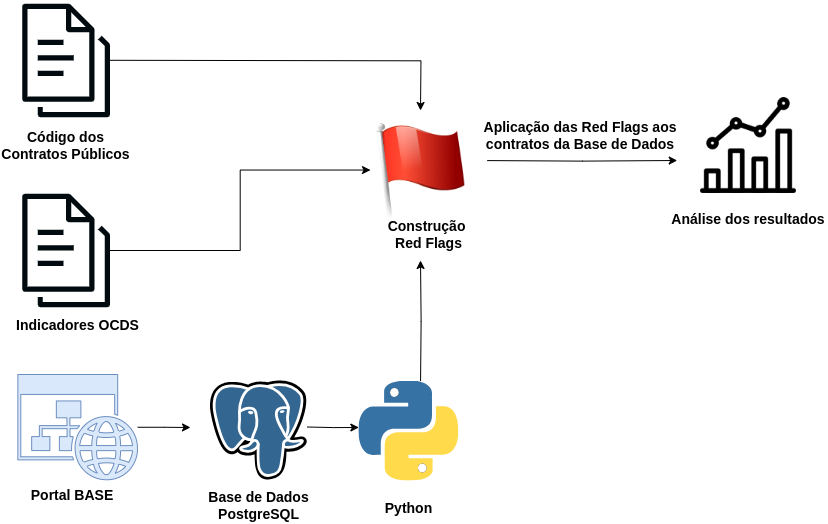
\includegraphics[width=0.85\textwidth]{imagens/processo_tese.png}
	\caption{Ilustração do conjunto de etapas envolvidas na elaboração do presente projeto. }
	\label{fig:processo}
\end{figure}

Ao longo deste texto, para todos os números referentes a valores pecuniários dos itens apresentados, o separador decimal será representado por vírgula e o separador dos milhares por ponto. Assim, o valor $20.315,42$ € corresponde a vinte mil, trezentos e quinze euros e quarenta e dois cêntimos. 

O desenvolvimento em software foi feito recorrendo à linguagem de programação Python (versão 3.11.8), ao sistema gerenciador de base de dados PostgreSQL (versão 8.1), à plataforma de controlo de versão Github, ao sistema de \textit{containerization} Docker (versão 25.0.3) e ao serviço de \textit{cloud} AWS. 


























































\section{Organização da tese}

Este relatório é composto por sete capítulos e encontram-se organizados da seguinte forma: 

\begin{my_itemize}


	\item \textbf{Capítulo 1 - Introdução}. Nesta capítulo é definido o problema que se pretende resolver, qual a necessidade em resolvê-lo o procedimento e os moldes em que se executou. Por fim, é apresentada a organização do presente relatório. 
	
	
	\item \textbf{Capítulo 2 - Contratação Pública em Portugal}. Neste capítulo é feita uma apresentação do Código dos Contratos Públicos em Portugal, onde são apresentados os principais objetivos deste documento e definidos os procedimentos e constituintes da formação de um contrato público.

	
	\item \textbf{Capítulo 3 - Noções Matemáticas}. Neste capítulo são apresentadas ferramentas básicas de Estatística, utilizadas recorrentemente na análise de dados. É apresentada a noção geral de \textit{outlier} e uma alternativa de deteção para distribuições assimétricas.

	
	\item \textbf{Capítulo 4 - Base de Dados}. Este capítulo encontra-se dividido em duas partes. Na primeira parte é descrito o \textit{website} de onde são recolhidos os dados, como é que o mesmo se encontra estruturado e as entidades envolvidas na regulação do mesmo. Na segunda parte é descrita a base de dados, como funciona o processo de recolha de dados, quais as colunas que revelaram maior interesse ao longo do desenvolvimento do projeto e a organização dos dados consoante diferentes variáveis de interesse, tais como o tipo de procedimento, valor adjudicado, categoria do contrato e local de execução.


	\item \textbf{Capítulo 5 - Aplicação de \textit{Red Flags}}. No início deste capítulo começa-se por apresentar o método de seleção de \textit{red flags}. De seguida, são caracterizadas as tabelas auxiliares da base de dados utilizadas ao longo do processo de construção das \textit{flags}. Por fim, é descrito o processo de construção de cada uma das flags desenvolvidas ao longo deste estágio e apresentados resultados após aplicação das mesmas.

	
	\item \textbf{Capítulo 6 - Processo de Automação}. Neste capítulo é descrito o processo de automação recorrendo à ferramenta de \textit{containerization} Docker e o serviço de \textit{cloud} AWS.

	
	\item \textbf{Capítulo 7 - Conclusão}. Por fim, neste capítulo, são sumariadas principais conclusões retiradas finda a construção e aplicação das \textit{red flags}, bem como possíveis melhorias e desenvolvimentos a serem considerados futuramente. 


\end{my_itemize}




